\documentclass[
11pt, % The default document font size, options: 10pt, 11pt, 12pt
%codirector, % Uncomment to add a codirector to the title page
]{charter} 


% El títulos de la memoria, se usa en la carátula y se puede usar el cualquier lugar del documento con el comando \ttitle
\titulo{Detección de anomalías en servicio de TV-over-IP mediante autoencoder LSTM} 

% Nombre del posgrado, se usa en la carátula y se puede usar el cualquier lugar del documento con el comando \degreename
%\posgrado{Carrera de Especialización en Sistemas Embebidos} 
%\posgrado{Carrera de Especialización en Internet de las Cosas} 
\posgrado{Carrera de Especialización en Inteligencia Artificial}
%\posgrado{Maestría en Sistemas Embebidos} 
%\posgrado{Maestría en Internet de las cosas}

% Tu nombre, se puede usar el cualquier lugar del documento con el comando \authorname
% IMPORTANTE: no omitir titulaciones ni tildación en los nombres, también se recomienda escribir los nombres completos (tal cual los tienen en su documento)
\autor{Ing. Christopher Charaf}

% El nombre del director y co-director, se puede usar el cualquier lugar del documento con el comando \supname y \cosupname y \pertesupname y \pertecosupname
\director{Título y Nombre del director}
\pertenenciaDirector{buscando} 
\codirector{} % para que aparezca en la portada se debe descomentar la opción codirector en los parámetros de documentclass
\pertenenciaCoDirector{FIUBA}

% Nombre del cliente, quien va a aprobar los resultados del proyecto, se puede usar con el comando \clientename y \empclientename
\cliente{Kaltura Inc.}
\empresaCliente{Kaltura Inc.}
 
\fechaINICIO{24 de junio de 2025}		%Fecha de inicio de la cursada de GdP \fechaInicioName
\fechaFINALPlan{20 de Octubre de 2025} 	%Fecha de final de cursada de GdP
\fechaFINALTrabajo{15 de diciembre de 2025}	%Fecha de defensa pública del trabajo final


\begin{document}

\maketitle
\thispagestyle{empty}
\pagebreak


\thispagestyle{empty}
{\setlength{\parskip}{0pt}
\tableofcontents{}-
}
\pagebreak


\section*{Registros de cambios}
\label{sec:registro}


\begin{table}[ht]
\label{tab:registro}
\centering
\begin{tabularx}{\linewidth}{@{}|c|X|c|@{}}
\hline
\rowcolor[HTML]{C0C0C0} 
Revisión & \multicolumn{1}{c|}{\cellcolor[HTML]{C0C0C0}Detalles de los cambios realizados} & Fecha      \\ \hline
0      & Creación del documento                                 &\fechaInicioName \\ \hline
1      & Se completa hasta el punto 5 inclusive                & 7 de Julio de 2025 \\ \hline
2      & Se completa hasta el punto 9 inclusive     & 15 de Julio de 2025 \\ \hline
%		  Se puede agregar algo más \newline
%		  En distintas líneas \newline
%		  Así                                                    & {día} de {mes} de 202X \\ \hline
3      & Se completa hasta el punto 12 inclusive                & 29 de Julio de 2025 \\ \hline
%4      & Se completa el plan	                                 & {día} de {mes} de 202X \\ \hline

% Si hay más correcciones pasada la versión 4 también se deben especificar acá

\end{tabularx}
\end{table}

\pagebreak



\section*{Acta de constitución del proyecto}
\label{sec:acta}

\begin{flushright}
Buenos Aires, \fechaInicioName
\end{flushright}

\vspace{2cm}

Por medio de la presente se acuerda con el \authorname\hspace{1px} que su Trabajo Final de la \degreename\hspace{1px} se titulará ``\ttitle'' y consistirá en la implementación de un sistema de detección de anomalías en un servicio de TV-over-IP mediante un autoencoder LSTM. El trabajo tendrá un presupuesto preliminar estimado de 600 horas y un costo estimado de \$ 1.420.000, con fecha de inicio el \fechaInicioName\hspace{1px} y fecha de presentación pública en el mes de diciembre de 2025.

Se adjunta a esta acta la planificación inicial.

\vfill

% Esta parte se construye sola con la información que hayan cargado en el preámbulo del documento y no debe modificarla
\begin{table}[ht]
\centering
\begin{tabular}{ccc}
\begin{tabular}[c]{@{}c@{}}Dr. Ing. Ariel Lutenberg \\ Director posgrado FIUBA\end{tabular} & \hspace{2cm} & \begin{tabular}[c]{@{}c@{}}\clientename \\ \empclientename \end{tabular} \vspace{2.5cm} \\ 
\multicolumn{3}{c}{\begin{tabular}[c]{@{}c@{}} \supname \\ Director del Trabajo Final\end{tabular}} \vspace{2.5cm} \\
\end{tabular}
\end{table}




\section{1. Descripción técnica-conceptual del proyecto a realizar}
\label{sec:descripcion}

El presente proyecto tiene como objetivo desarrollar un sistema de detección de anomalías en tiempo real aplicado a un servicio de televisión por protocolo de Internet (TV-over-IP) basado en interfaces de programación de aplicaciones (API). Este servicio es monitoreado mediante métricas recolectadas a través de una herramienta de acumulacion de métricas llamada Prometheus, con una frecuencia de muestreo de 30 segundos. El sistema propuesto busca identificar comportamientos inusuales o fallos en el servicio mediante la reconstrucción de secuencias de métricas utilizando un modelo Autoencoder basado en redes neuronales de memoria a largo y corto plazo (LSTM, por sus siglas en inglés: \textit{Long Short-Term Memory}).

La empresa cliente dee este proyecto es "Kaltura Inc.", la cual provee servicios de TV-over-IP sobre infraestructura en la nube de Amazon Web Services (AWS). Esta empresa se enfrenta al desafío creciente de modernizar sus herramientas de monitoreo para mejorar la capacidad de reacción ante fallos en producción, sin depender exclusivamente de soluciones externas. Por este motivo, este desarrollo responde a una necesidad concreta del área de operaciones y calidad de servicio de la organización frente a sus clientes.

Actualmente, los métodos tradicionales de monitoreo utilizan umbrales fijos o alertas manuales, lo cual resulta ineficiente frente a comportamientos no triviales o patrones de uso dinámicos. Además, muchas herramientas de monitoreo de terceros requieren la exposición de métricas internas a servicios externos, por lo que compromete  la privacidad de los datos y aumenta la propensión a ataques. En contraste, este proyecto propone una solución propietaria, basada en aprendizaje automático, que permita detectar anomalías de manera autónoma, no invasiva y segura.

Desde el punto de vista técnico, el modelo recibirá como entrada ventanas deslizantes de tiempo compuestas por un número a definir de métricas técnicas que reflejan el rendimiento del servicio en tiempo real. Se utilizarán técnicas de ingeniería de características (\textit{feature engineering}) como la codificación cíclica del horario y variables contextuales que representen ventanas de mantenimiento y fines de semana para mejorar la sensibilidad del modelo frente a patrones estacionales.

Se empleará una arquitectura LSTM Autoencoder que aprende a reconstruir secuencias temporales multivariadas. Si el error de reconstrucción excede un umbral previamente definido, se considera que ocurrió una anomalía. En caso de detección, se emitirán alertas automáticas a través de la plataforma de alertas Opsgenie y se generarán enlaces a paneles de visualización de métricas como Grafana con el contexto temporal de la anomalía.

Esta propuesta se encuentra actualmente en su etapa inicial de planeamiento, donde se están definiendo tanto la arquitectura del modelo como las herramientas de integración con el ecosistema de monitoreo ya existente. La innovación principal reside en la aplicación de redes neuronales recurrentes para detección de anomalías directamente dentro del entorno técnico de la empresa, sin depender de soluciones comerciales de terceros. Esto refuerza la privacidad de los datos sensibles del sistema y de los usuarios, y permite una mayor adaptabilidad a los cambios en el comportamiento del servicio.

En comparación con el estado del arte, esta solución se destaca por su enfoque específico a servicios basados en API en tiempo real, su integración directa con herramientas de acumulación de métricas Prometheus y Grafana y por aplicar técnicas avanzadas de aprendizaje profundo en lugar de reglas estáticas. Esto la convierte en una alternativa más precisa, segura, escalable y personalizada que herramientas convencionales de detección de anomalías y alertas nativas de Grafana.

Cabe mencionar que no existen fuentes de financiamiento externo ni convenios públicos involucrados. El proyecto se desarrolla como parte del trabajo profesional del autor, y de acuerdo con el contrato vigente con la empresa, la propiedad intelectual de todos los entregables pertenece a la organización.

El cliente interno de este desarrollo es el área de operaciones de la empresa, que valora especialmente la capacidad de detección proactiva de incidentes, la integración fluida con su infraestructura existente y la reducción de falsos positivos. Necesita una solución confiable, sustentable y alineada con sus políticas de seguridad.

En la figura 1 se presenta el diagrama en bloques del sistema. Se observa que el flujo de datos comienza con la recolección de métricas desde Prometheus a través de su API, las cuales se almacenan en un marco de datos (\textit{dataframe}) y luego se someten a un proceso de preprocesamiento e ingeniería de características. A continuación, estas métricas son introducidas en un modelo Autoencoder basado en redes LSTM, compuesto por un codificador (\textit{encoder}) y un decodificador (\textit{decoder}), que tiene como objetivo reconstruir la secuencia original de datos. El sistema evalúa el error de reconstrucción de dichas métricas y lo compara contra un umbral definido: si el error excede dicho umbral, se considera que ocurrió una anomalía. En ese caso, se dispara una alerta automática hacia Opsgenie y se genera un enlace contextual hacia un panel de visualización en Grafana, lo que permite al equipo de operaciones inspeccionar el evento detectado con información visual en tiempo real. 

Si no se detecta anomalía, el sistema continúa procesando los siguientes datos de forma continua y en tiempo real. 

 

\begin{figure}[htpb]
\centering 
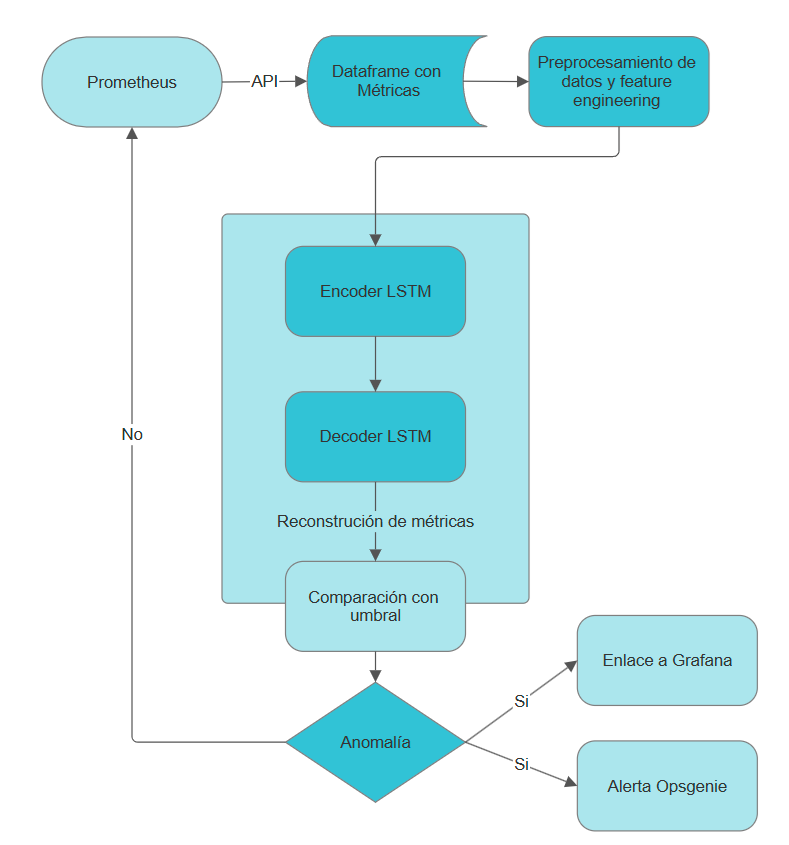
\includegraphics[width=.65\textwidth]{./Figuras/diag.png}
\caption{Diagrama en bloques del sistema.}
\label{fig:diagBloques}
\end{figure}

\vspace{25px}

\section{2. Identificación y análisis de los interesados}
\label{sec:interesados}
\begin{table}[ht]
%\caption{Identificación de los interesados}
%\label{tab:interesados}
\begin{tabularx}{\linewidth}{@{}|l|X|X|l|@{}}
\hline
\rowcolor[HTML]{C0C0C0} 
Rol           & Nombre y Apellido & Organización 	& Puesto 	\\ \hline
Auspiciante   &           Sergio Sancho        &  \clientename             	&      Ingeniero de soporte  	\\ \hline
Responsable   & \authorname       & FIUBA        	& Alumno 	\\ \hline
Orientador    & \supname	      & \pertesupname 	& Director del trabajo final \\ \hline
Usuario final &       \clientename            &         \clientename     	&   Departamento de soporte y operaciones     	\\ \hline
\end{tabularx}
\end{table}


\begin{itemize}
	\item Orientador: a definir.
	\item Auspiciante: será el mismo usuario final de la solución, valora costos y organización en los procesos automatizados. 
\end{itemize}


\section{3. Propósito del proyecto}
\label{sec:proposito}
El propósito del proyecto es diseñar e implementar un sistema inteligente que permita detectar anomalías en tiempo real dentro de un servicio de televisión por protocolo de \textit{Internet} (\textit{TV-over-IP}), basado en APIs y desplegado sobre infraestructura en la nube. Mediante el uso de un modelo \textit{autoencoder} basado en redes neuronales LSTM, se busca brindar a la empresa una herramienta robusta y segura para el monitoreo continuo de métricas técnicas clave; esta solución mejora su capacidad de respuesta ante incidentes, minimiza el tiempo de inactividad del servicio y garantiza una mayor calidad de experiencia para sus usuarios finales. 

\section{4. Alcance del proyecto}
\label{sec:alcance}

El proyecto incluye:
\begin{itemize}
    \item La definición y análisis de métricas críticas del servicio de TV-over-IP recolectadas desde Prometheus mediante su API.
    \item El diseño e implementación de una serie de procesos(\textit{pipeline}) de procesamiento de datos, incluyendo:
    \begin{itemize}
        \item Normalización de variables.
        \item \textit{Feature engineering} (codificación cíclica de hora, día, etc.).
        \item Construcción de ventanas deslizantes para series temporales.
    \end{itemize}
    \item El desarrollo de un modelo de detección de anomalías basado en Autoencoder LSTM, entrenado para reconstruir secuencias multivariadas normales.
    \item La integración del sistema con herramientas de monitoreo existentes:
    \begin{itemize}
        \item Generación de alertas automáticas vía Opsgenie.
        \item Enlace contextual a paneles de Grafana.
    \end{itemize}
    \item La validación del sistema en un entorno de producción con datos reales históricos.
    \item La elaboración de documentación técnica y funcional del prototipo.
\end{itemize}
El presente proyecto no incluye:

\begin{itemize}
    \item El desarrollo de interfaces gráficas adicionales fuera de Grafana.
    \item La implementación de acciones correctivas automáticas posteriores a la detección de anomalías.
    \item La gestión directa de recursos en AWS ni tareas de infraestructura subyacente (como escalado automático, balanceo de carga, etc.).
\end{itemize}



\section{5. Supuestos del proyecto}
\label{sec:supuestos}

Para el desarrollo del presente proyecto se supone que:

\begin{enumerate}
    \item \clientename  \space brindará acceso a las métricas necesarias a través de su instancia de Prometheus mediante API REST, así como también a sus paneles de visualización en Grafana.
    \item El \textit{dataframe} histórico utilizado para entrenamiento estará disponible, completo y será representativo del comportamiento normal del sistema en condiciones reales de operación.
    \item Se contará con los recursos computacionales necesarios (por ejemplo, GPU opcional) para el entrenamiento del modelo LSTM Autoencoder en un entorno controlado por \clientename.
    \item Las herramientas de integración como Opsgenie y Grafana ya están operativas y disponibles para pruebas dentro de la infraestructura de la empresa.
    \item No se producirán cambios drásticos en el comportamiento del servicio durante el período de entrenamiento y validación que comprometan la utilidad del modelo.
    \item El equipo de operaciones colaborará en la validación funcional del sistema, especialmente en la evaluación de falsos positivos y en el ajuste del umbral de alerta en base a estándares existentes en la empresa.
    \item Las condiciones legales, de seguridad y de confidencialidad establecidas en el contrato del autor con la empresa se mantendrán vigentes y permitirán el desarrollo del proyecto sin restricciones externas.
\end{enumerate}


\section{6. Requerimientos}
\label{sec:requerimientos}


\begin{enumerate}
    \item Requerimientos\textbf{ }funcionales:
 1.1. El sistema debe ser capaz de recolectar métricas técnicas desde Prometheus a través de su API REST. (Alta prioridad)

 1.2. El sistema debe construir ventanas deslizantes de 20 pasos temporales (10 minutos) con una frecuencia de muestreo de 30 segundos. (Alta prioridad)

 1.3. El sistema debe aplicar técnicas de normalización y codificación cíclica de variables temporales como \verb|hour_sin| y \verb|hour_cos|. (Alta prioridad)

 1.4. El modelo debe reconstruir secuencias multivariadas. (Alta prioridad)

 1.5. El sistema debe detectar anomalías cuando el error de reconstrucción supere un umbral configurable. (Alta prioridad)

 1.6. En caso de anomalía, el sistema debe enviar una alerta automática a través de Opsgenie. (Media prioridad)

 1.7. El sistema debe incluir un enlace a Grafana que muestre el contexto temporal de la anomalía detectada. (Media prioridad)
    \item Requerimientos de documentación:

 2.1. Se debe entregar documentación técnica del modelo, su entrenamiento, configuración y uso. (Alta prioridad)

 2.2. Se debe entregar una memoria del trabajo final con descripción funcional, arquitectura y resultados. (Alta prioridad)

 2.3. Se debe incluir una guía básica de despliegue e integración del sistema en entornos compatibles. (Media prioridad)
    \item Requerimientos de \textit{testing} y validación:

 3.1. El sistema debe ser validado sobre datos históricos que representen el comportamiento normal del sistema. (Alta prioridad)

 3.2. Se deben generar métricas de desempeño como tasa de falsos positivos y precisión de detección. (Alta prioridad)

 3.3. El umbral de error debe ser calibrado en conjunto con el equipo de operaciones. (Media prioridad)
    \item Requerimientos de interfaz:

 4.1. El sistema no debe contar con una interfaz gráfica propia, pero debe integrarse con visualizaciones (\textit{dashboards}) existentes en Grafana. (Alta prioridad)

 4.2. El mensaje de alerta debe incluir timestamp, métricas anómalas, y visualización de valores reales vs reconstruidos. (Media prioridad)
    \item Requerimientos de interoperatividad e integración:

 5.1. El sistema debe integrarse con la instancia de Prometheus de la empresa. (Alta prioridad)

 5.2. El sistema debe ser compatible con Grafana para visualización. (Alta prioridad)

 5.3. El sistema debe ser capaz de emitir alertas en el formato requerido por Opsgenie. (Media prioridad)
    \item Requerimientos normativos y de seguridad:

 6.1. El sistema no debe enviar datos a servicios externos no autorizados. (Alta prioridad)

 6.2. Todo el procesamiento debe realizarse dentro de la red interna de la empresa o su infraestructura autorizada en AWS. (Alta prioridad)

 6.3. El sistema debe respetar las políticas internas de privacidad y seguridad de la información establecidas por la empresa. (Alta prioridad)
    \item Requerimientos opcionales:

 7.1. Incluir variables adicionales como \verb|weekday|, \verb|is_weekend|, \verb|is_night| en el \textit{feature engineering}. (Opcional)

 7.2. Permitir ajuste dinámico del umbral de detección desde una configuración externa. (Opcional) 
\end{enumerate}
   
    
\section{7. Historias de usuarios (\textit{Product backlog})}
\label{sec:backlog}

Los story points se asignaron considerando tres factores:

\begin{itemize}
    \item Complejidad técnica (1 a 5)
    \item Dificultad de implementación (1 a 5)
    \item Grado de incertidumbre (1 a 5)

 Fórmula: SP = Complejidad + Dificultad + Incertidumbre
\end{itemize}

\begin{enumerate}
    \item “Como ingeniero de monitoreo quiero recibir alertas automáticas cuando se detecten anomalías para poder reaccionar rápidamente y minimizar el impacto en el servicio.”

 Story points: 8 (Complejidad: 3, Dificultad: 2, Incertidumbre: 3)
    \item “Como desarrollador de datos quiero procesar las métricas recolectadas y convertirlas en secuencias temporales con variables adicionales para entrenar el modelo.”

 Story points\textbf{:} 7 (Complejidad: 3, Dificultad: 2, Incertidumbre: 2)
    \item “Como operador del sistema quiero que cada alerta contenga un enlace directo a un panel de Grafana para visualizar rápidamente la anomalía detectada.”

 Story points\textbf{:} 5 (Complejidad: 2, Dificultad: 1, Incertidumbre: 2)
    \item “Como responsable de infraestructura quiero que el sistema funcione dentro de nuestra red privada para evitar exponer datos sensibles a servicios externos.”

 Story points: 6 (Complejidad: 2, Dificultad: 2, Incertidumbre: 2)
    \item “Como científico de datos quiero entrenar el modelo sobre datos históricos para que aprenda el comportamiento normal del sistema.”

 Story points\textbf{:} 6 (Complejidad: 2, Dificultad: 2, Incertidumbre: 2)
    \item “Como técnico de soporte quiero acceder a un log con las métricas reales y reconstruidas al momento de la anomalía para facilitar el diagnóstico del incidente.”

 Story points\textbf{:} 5 (Complejidad: 2, Dificultad: 2, Incertidumbre: 1)
\end{enumerate}


\section{8. Entregables principales del proyecto}
\label{sec:entregables}

\begin{itemize}
    \item Documentación técnica del sistema:

 Contendrá la descripción de la arquitectura del modelo, el flujo de procesamiento de datos, los componentes implementados y las herramientas utilizadas (Prometheus, Grafana, Opsgenie, entre otras).
    \item Memoria del trabajo final:

 Documento completo que incluye la descripción técnica-conceptual, estado del arte, objetivos, metodología, implementación, resultados obtenidos y conclusiones.
    \item Código fuente del sistema:

 Scripts y módulos desarrollados para el procesamiento de datos, entrenamiento del modelo, inferencia y generación de alertas. El código será entregado con instrucciones de ejecución y dependencias requeridas.
    \item Modelo LSTM Autoencoder entrenado:

 Archivo con los pesos y la estructura del modelo entrenado, listo para su despliegue en entorno de validación o producción.
    \item Pipeline de procesamiento de datos:

 Conjunto de scripts que automatizan las etapas de recolección, transformación, normalización y estructuración de datos históricos en secuencias para el modelo.
    \item Configuración de integración con Opsgenie y Grafana:

 Archivos de configuración, ejemplos y plantillas para la conexión del sistema con los mecanismos de alerta y visualización en tiempo real utilizados por la empresa.
 \item Informe de avances:

Entregable requerido por la carrera de especialización que resume el estado del proyecto durante su desarrollo.
\end{itemize}
    

\section{9. Desglose del trabajo en tareas}
\label{sec:wbs}

\begin{enumerate}
\item Análisis y definición del sistema (70 h)
\begin{enumerate}
  \item Revisión del estado del arte y casos similares (15 h)
  \item Análisis de métricas disponibles en Prometheus (20 h)
  \item Definición de requerimientos funcionales y no funcionales (20 h)
  \item Diseño preliminar del sistema y definición del pipeline (15 h)
\end{enumerate}
\item Desarrollo del pipeline de datos (100 h)
\begin{enumerate}
  \item Implementación del recolector de métricas desde Prometheus (20 h)
  \item Desarrollo de preprocesamiento y normalización (25 h)
  \item Implementación de ingeniería de variables temporales (20 h)
  \item Construcción de ventanas deslizantes para series temporales (20 h)
  \item Validación del pipeline con datos históricos (15 h)
\end{enumerate}
\item Desarrollo y entrenamiento del modelo (150 h)
\begin{enumerate}
  \item Definición de arquitectura LSTM Autoencoder (20 h)
  \item Implementación del modelo en Keras/TensorFlow (30 h)
  \item Preparación del conjunto de entrenamiento y validación (20 h)
  \item Entrenamiento del modelo con tuning de hiperparámetros (45 h)
  \item Evaluación del desempeño con métricas objetivas (35 h)
\end{enumerate}
\item Integración con sistema de monitoreo (Grafana y Opsgenie) (90 h)
\begin{enumerate}
  \item Diseño del mecanismo de alerta con umbral configurable (25 h)
  \item Integración con Opsgenie para envío de alertas (20 h)
  \item Generación de enlaces hacia dashboards de Grafana (15 h)
  \item Pruebas de integración en entorno controlado (30 h)
\end{enumerate}
\item Validación, documentación y entregables (190 h)
\begin{enumerate}
  \item Validación funcional con el equipo de operaciones (25 h)
  \item Elaboración del informe de resultados y validación (20 h)
  \item Redacción de la memoria técnica (1° bimestre) (40 h)
  \item Redacción de la memoria técnica (2° bimestre) (40 h)
  \item Preparación de documentación de uso e integración (25 h)
  \item Informe de avances (requerido por la especialización) (20 h)
  \item Elaboración y ensayo de presentación final (20 h)
\end{enumerate}
\end{enumerate}

\textbf{Cantidad total de horas: 600 h.}


\section{10. Diagrama de Activity On Node}
\label{sec:AoN}

\begin{table}[H]
\centering
\begin{tabular}{|>{\centering\arraybackslash}p{0.17\linewidth}|>{\raggedright\arraybackslash}p{0.33\linewidth}|>{\raggedright\arraybackslash}p{0.5\linewidth}|}
\hline
\rowcolor[HTML]{EFEFEF}
\textbf{Color} & \textbf{Grupo de tareas} & \textbf{Descripción} \\ \hline

\cellcolor[HTML]{FFF2CC} Amarillo claro & Grupo 1: análisis y definición del sistema& Tareas relacionadas con el estudio preliminar, análisis de métricas, requisitos y diseño inicial. \\ \hline

\cellcolor[HTML]{DAE8FC} Celeste claro & Grupo 2: desarrollo del pipeline de datos& Implementación del recolector de métricas, preprocesamiento, normalización y ventanas deslizantes. \\ \hline

\cellcolor[HTML]{E1D5E7} Violeta claro & Grupo 3: desarrollo y entrenamiento del modelo& Definición de la arquitectura, implementación y evaluación del modelo LSTM Autoencoder. \\ \hline

\cellcolor[HTML]{F8CECC} Rosado claro & Grupo 4: integración con sistema de monitoreo& Tareas de conexión con Opsgenie, configuración de alertas y enlaces hacia dashboards de Grafana. \\ \hline

\cellcolor[HTML]{D5E8D4} Verde claro & Grupo 5: validación, documentación y entregables& Actividades de verificación, redacción del informe técnico y documentación final del proyecto. \\ \hline

\cellcolor[HTML]{FFFFFF} Blanco & Inicio / Fin & Representa los nodos de comienzo y cierre del proyecto. \\ \hline

\end{tabular}
\caption{Cuadro indicativo de colores del Diagrama AoN.}
\end{table}


\begin{figure}[htpb]
\centering 
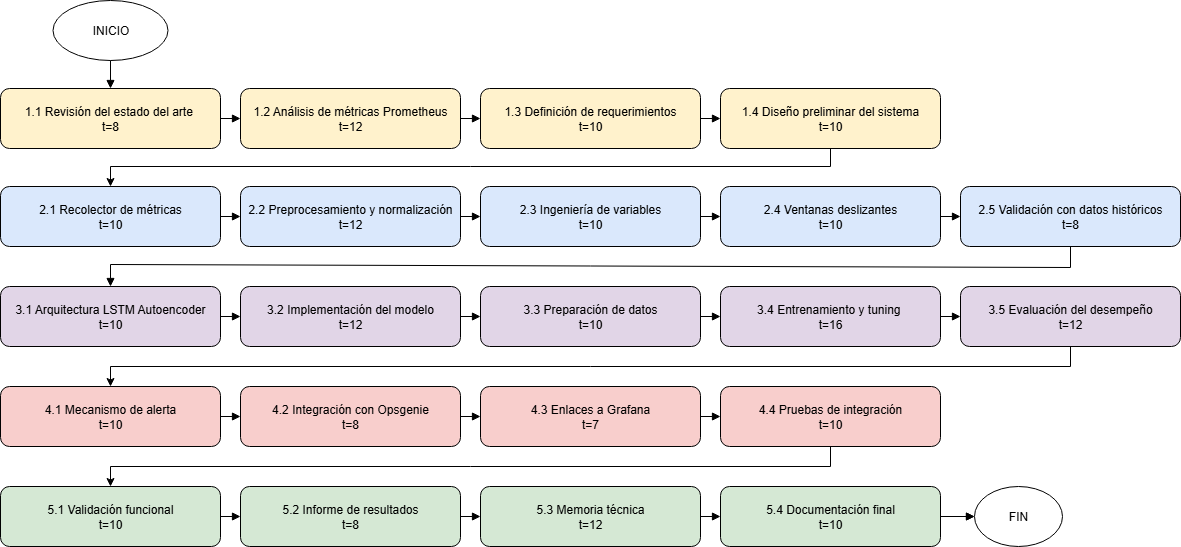
\includegraphics[width=1\textwidth]{./Figuras/AoN.png}
\caption{Diagrama de \textit{Activity on Node}.}
\label{fig:AoN}
\end{figure}



\section{11. Diagrama de Gantt}
\label{sec:gantt}
A continuación se presenta el diagrama de Gantt correspondiente al cronograma del proyecto. El mismo se muestra en formato apaisado con el objetivo de facilitar su lectura y visualización el cual permite apreciar con claridad la secuencia temporal de las actividades planificadas, su duración estimada y su relación con el resto de las tareas. Este diagrama fue elaborado en base al desglose de tareas definido en el WBS (punto 9) y refleja la distribución efectiva del trabajo a lo largo del tiempo, considerando una carga de 6 horas diarias, días no laborables y períodos de vacaciones. 
\begin{landscape}
\begin{figure}[H]
\centering
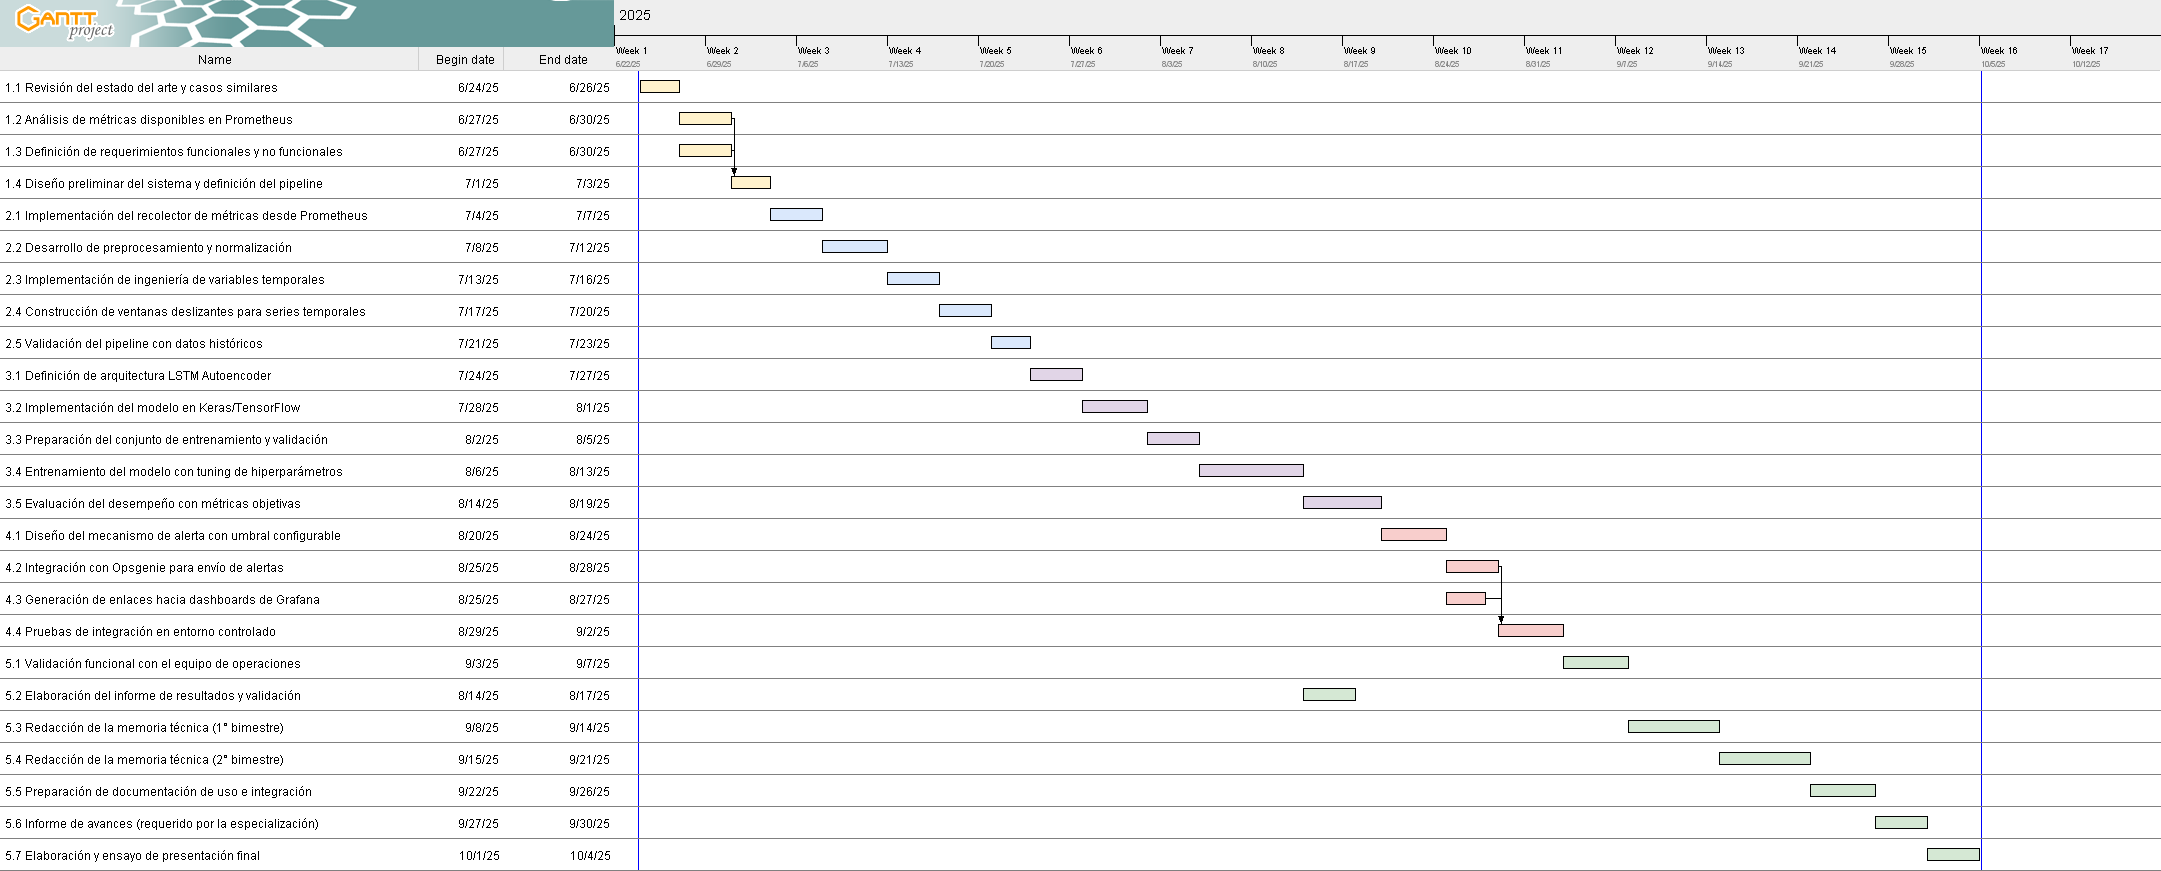
\includegraphics[width=\linewidth,keepaspectratio]{./Figuras/Gantt-2.png}
\caption{Diagrama de Gantt (apaisado).}
\label{fig:diagGantt}

\end{figure}
\end{landscape}



\section{12. Presupuesto detallado del proyecto}
\label{sec:presupuesto}

\begin{table}[H]
\centering
\begin{tabular}{|>{\raggedright\arraybackslash}p{0.25\linewidth}|>{\centering\arraybackslash}p{0.25\linewidth}|>{\centering\arraybackslash}p{0.25\linewidth}|>{\centering\arraybackslash}p{0.25\linewidth}|}
\hline
\textbf{Descripción} & \textbf{Cantidad (h)} & \textbf{Valor unitario (ARS)} & \textbf{Valor total (ARS)} \\
\hline
Análisis y definición del sistema & 70 & 2.250 & 157.500 \\\hline
Desarrollo del pipeline de datos  & 95 & 2.250 & 213.750 \\\hline
Desarrollo y entrenamiento del modelo & 125 & 2.250 & 281.250 \\\hline
Integración con herramientas de monitoreo & 90 & 2.250 & 202.500 \\\hline
Validación, documentación y entregables & 120 & 2.250 & 270.000 \\
\hline
\textbf{Subtotal costos directos} & \textbf{600} &  & \textbf{1.350.000} \\
\hline
\end{tabular}
\caption{Presupuesto de costos directos del proyecto.}
\end{table}

\vspace{0.5cm}

\begin{table}[H]
\centering
\begin{tabular}{|>{\raggedright\arraybackslash}p{0.25\linewidth}|>{\centering\arraybackslash}p{0.25\linewidth}|>{\centering\arraybackslash}p{0.25\linewidth}|>{\centering\arraybackslash}p{0.25\linewidth}|}
\hline
\textbf{Descripción} & \textbf{Cantidad} & \textbf{Valor unitario (ARS)} & \textbf{Valor total (ARS)} \\
\hline
Electricidad y conectividad (mensual estimado) & 3 meses & 15.000 & 45.000 \\\hline
Licencias de software y servicios en la nube (AWS) & 1 uso & 25.000 & 25.000 \\
\hline
\textbf{Subtotal costos indirectos} &  &  & \textbf{70.000} \\
\hline
\end{tabular}
\caption{Presupuesto de costos indirectos del proyecto.}
\end{table}

\vspace{0.5cm}

\noindent\textbf{Costo total del proyecto: \quad 1.420.000 ARS}


\newpage



\section{13. Gestión de riesgos}
\label{sec:riesgos}

\subsection*{a) Identificación de los riesgos}

Riesgo 1: Retrasos por disponibilidad limitada de recursos computacionales en AWS \\
Severidad (S): 8. Puede impactar directamente el entrenamiento del modelo y postergar hitos clave. \\
Ocurrencia (O): 6. Es posible durante el uso compartido de cuentas gratuitas o cuotas restringidas en nube.

\vspace{0.2cm}
Riesgo 2: Baja calidad o inconsistencias en los datos históricos \\
Severidad (S): 7. Afectaría la capacidad de generalización del modelo y su precisión. \\
Ocurrencia (O): 5. Dado que Prometheus no garantiza calidad semántica, existe una probabilidad media.

\vspace{0.2cm}
Riesgo 3: Alta tasa de falsos positivos en producción \\
Severidad (S): 9. Daña la confiabilidad del sistema y satura al equipo de operaciones. \\
Ocurrencia (O): 4. Aunque el modelo será entrenado cuidadosamente, es una posibilidad al inicio.

\vspace{0.2cm}
Riesgo 4: Retrasos en la integración con herramientas externas (Grafana / Opsgenie) \\
Severidad (S): 6. Afecta el valor operativo del sistema si no puede emitir alertas. \\
Ocurrencia (O): 5. Existen APIs documentadas, pero pueden surgir problemas de permisos o conectividad.

\vspace{0.2cm}
Riesgo 5: Reentrenamiento frecuente por cambios en el comportamiento del servicio \\
Severidad (S): 5. Implica tareas adicionales no previstas si el modelo no se adapta. \\
Ocurrencia (O): 6. Dado que el tráfico de usuarios puede ser estacional o volátil.

\vspace{0.5cm}
\subsection*{b) Tabla de gestión de riesgos}

\begin{table}[H]
\centering
\begin{tabular}{|l|c|c|c|c|c|c|}
\hline
Riesgo & S & O & RPN & S* & O* & RPN* \\
\hline
1. Recursos en AWS & 8 & 6 & 48 & 6 & 4 & 24 \\\hline
2. Calidad de datos & 7 & 5 & 35 & 6 & 4 & 24 \\\hline
3. Falsos positivos & 9 & 4 & 36 & 6 & 3 & 18 \\\hline
4. Integración externa & 6 & 5 & 30 & 5 & 3 & 15 \\\hline
5. Cambios en patrones & 5 & 6 & 30 & 4 & 4 & 16 \\
\hline
\end{tabular}
\caption{Tabla de gestión de riesgos del proyecto.}
\end{table}

\vspace{0.2cm}
Criterio adoptado: Se tomarán medidas de mitigación para los riesgos con RPN mayor a 30.

\vspace{0.5cm}
\subsection*{c) Plan de mitigación}

Riesgo 1 – Recursos computacionales en AWS: \\
Mitigación: Uso de instancias locales para pruebas preliminares; reserva de tiempo para ventanas de entrenamiento. \\
Severidad (S*): 6. Porque las tareas críticas se reprograman con anticipación. \\
Ocurrencia (O*): 4. Menor dependencia tras balanceo entre recursos locales y en la nube.

\vspace{0.2cm}
Riesgo 2 – Calidad de datos históricos: \\
Mitigación: Auditoría inicial y filtrado de valores atípicos (outliers) en el preprocesamiento. \\
Severidad (S*): 6. Impacto reducido al depurar métricas poco confiables. \\
Ocurrencia (O*): 4. Menor probabilidad tras control manual previo al entrenamiento.

\vspace{0.2cm}
Riesgo 3 – Falsos positivos: \\
Mitigación: Ajuste de umbrales, evaluación del modelo con set de validación y revisión cruzada. \\
Severidad (S*): 6. No se eliminan del todo pero se reduce el impacto. \\
Ocurrencia (O*): 3. Tras ajuste de umbrales y revisión conjunta con operaciones.



\section{14. Gestión de la calidad}
\label{sec:calidad}

En la siguiente tabla se detallan diez requerimientos clave del proyecto, seleccionados por su criticidad, impacto funcional o valor para el adoptante final. Para cada uno de ellos se especifican los mecanismos de verificación (control técnico interno) y validación (desde la perspectiva del cliente u operador del sistema). Esto permite asegurar la calidad tanto técnica como operativa de los entregables.

\begin{table}[H]
\centering
\begin{tabular}{|p{4cm}|p{5cm}|p{5cm}|}
\hline
\textbf{Requerimiento} & \textbf{Verificación (caja blanca)} & \textbf{Validación (caja negra)} \\
\hline
1. El sistema debe detectar anomalías con datos multivariados & Evaluación de reconstrucción vs señal original usando error cuadrático medio (MSE) & Revisión funcional con el equipo de soporte sobre detecciones correctas e incorrectas\\
\hline
2. El modelo debe entrenarse correctamente con series históricas & Pruebas de entrenamiento supervisado y convergencia de la pérdida & Validación con datos históricos y validación cruzada sobre ventanas de tiempo reales \\
\hline
3. El sistema debe generar alertas automáticamente ante detección de anomalías & Test unitarios sobre el módulo de detección y umbrales configurables & Observación real en entorno de pre-producción; confirmación por parte del equipo de monitoreo\\
\hline
4. Integración con Opsgenie para envío de alertas & Simulación de alertas y verificación de contenidos enviados& Recepción correcta en panel de alertas y notificaciones por parte del equipo de soporte\\
\hline
5. Generación automática de enlaces hacia dashboards en Grafana & Verificación del formato correcto de URLs generadas dinámicamente & Acceso correcto y funcional desde la alerta hasta el dashboard relevante \\
\hline
6. Documentación técnica del modelo entrenado & Revisión de estructura técnica completa (modelo, inputs, outputs)& Validación por el equipo de infraestructura\\
\hline
7. Manual de usuario final para configuración del sistema & Revisión ortográfica y técnica& Validación con usuario final mediante prueba de instalación paso a paso \\
\hline
8. El sistema debe soportar nuevas métricas sin reentrenamiento completo & Prueba modular de inputs y vuelta a valores por defecto& Simulación de nuevas métricas por parte del equipo de monitoreo para validar robustez \\
\hline
9. Interoperabilidad con Prometheus como fuente de métricas & Testeo de conexión y recopilación de métricas a intervalos regulares& Verificación del flujo de datos en tiempo real dentro del dashboard de Grafana \\
\hline
10. El sistema debe ejecutarse como un servicio en segundo plano & Pruebas funcionales y logs operativos bajo supervisión& Validación por el equipo de infraestructura en entorno de producción \\
\hline
\end{tabular}
\caption{Gestión de calidad: verificación y validación de los principales requerimientos.}
\end{table}


\section{15. Procesos de cierre}    
\label{sec:cierre}


Una vez completadas todas las actividades planificadas en el proyecto, se llevará a cabo una reunión final de evaluación con el objetivo de formalizar su cierre. A continuación, se detallan las pautas de trabajo que guiarán dicho proceso:

\begin{itemize}
    \item Evaluación del cumplimiento del Plan de Proyecto\textbf{:}  
    La revisión del cumplimiento del plan original estará a cargo del lider técnico del equipo de soporte de la empresa. El procedimiento consistirá en contrastar el cronograma y el WBS definidos en las etapas iniciales con las tareas efectivamente ejecutadas, verificando desviaciones en duración, entregables y prioridades. Se utilizarán las versiones documentadas en Git o carpetas compartidas como evidencia del seguimiento.

    \item Análisis de técnicas, problemas y soluciones\textbf{:}  
    Se realizará una revisión retrospectiva sobre las técnicas empleadas, diferenciando aquellas que fueron eficaces (como el uso de Autoencoders LSTM para detección multivariada) de aquellas que resultaron inadecuadas o descartadas de otros modelos. También se documentarán los problemas surgidos (por ejemplo, calidad de datos, disponibilidad de infraestructura en la nube) y las estrategias aplicadas para resolverlos. Todo este análisis será consolidado y documentado pertinentemente.

    \item Acto de cierre y agradecimiento\textbf{:}  
    El acto de cierre será organizado por el autor del proyecto, quien se encargará de invitar y agradecer especialmente al equipo de operaciones, al personal técnico que colaboró en las etapas de validación, y a la empresa por su apoyo institucional. En caso de realizarse un pequeño evento informal o encuentro virtual, los gastos serán cubiertos personalmente por el responsable del proyecto, sin requerir financiamiento institucional adicional.
\end{itemize}

Estas acciones permitirán formalizar el cierre técnico y administrativo del proyecto, dejando trazabilidad de su cumplimiento, reconociendo a los colaboradores y consolidando el conocimiento generado.


\end{document}